\documentclass[17pt, t, lualatex]{beamer}

\title{The Imitation Game\\\large Teaching Computers to Imitate Neurons}
\date{March 15th, 2026}
\institute[KTH]{KTH Royal Institute of Technology}
\author{Paul Mayer}

\usepackage{amsmath,amssymb,mathtools}
\usepackage{hyperref}
\usepackage{booktabs}
\usepackage{tikz}
\usetikzlibrary{shapes,arrows,positioning,calc,decorations.pathreplacing}

% Probably load as late as possible
\usetheme[engine=lualatex, mathshape=sf, fontdir=kthpq-files/fonts/Figtree/]{kthpq}
\setmonofont{Bitstream Vera Sans Mono}[Scale=.9]

\begin{document}

\inserttitlepage

%% ============================================================
%% SLIDE 1: The Dream — Simulating the Brain
%% ============================================================
\begin{frame}{The Dream: Simulating the Brain}
\begin{center}
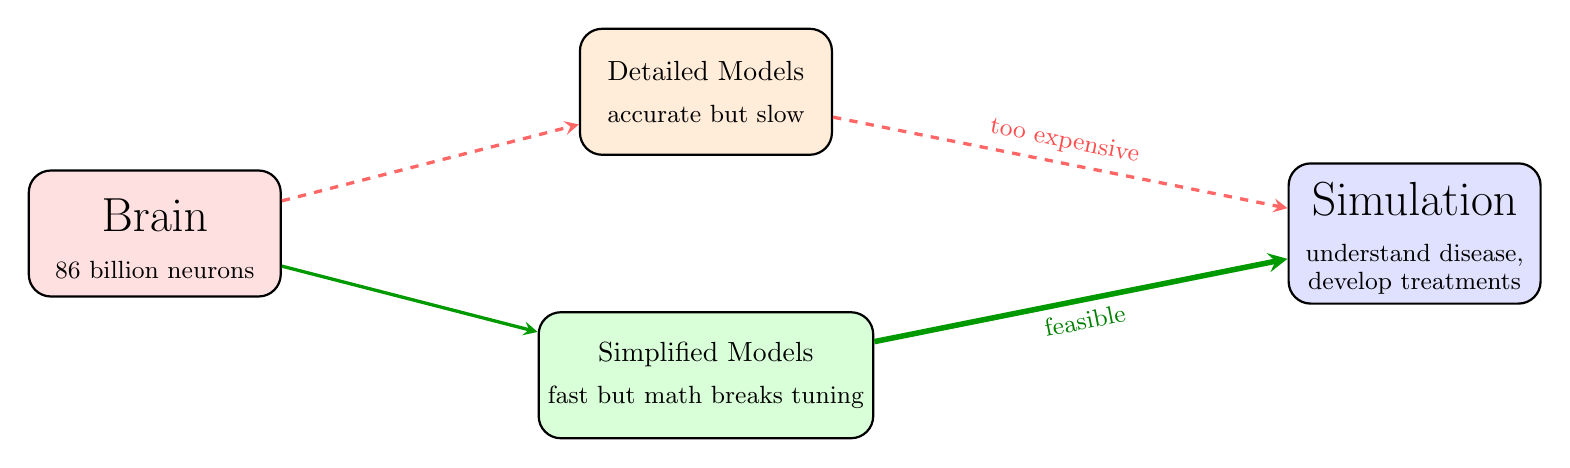
\begin{tikzpicture}[
    box/.style={draw, rounded corners=8pt, minimum width=3.2cm, minimum height=1.6cm,
                align=center, font=\normalsize, thick},
    arrow/.style={->, very thick, >=stealth}
]
    % Brain
    \node[box, fill=red!12] (brain) at (0,0) {
        \LARGE\strut Brain\\[3pt]
        \small 86 billion neurons
    };

    % Detailed models
    \node[box, fill=orange!15] (detail) at (7,1.8) {
        Detailed Models\\[3pt]
        \small accurate but slow
    };

    % Simplified models
    \node[box, fill=green!15] (simple) at (7,-1.8) {
        Simplified Models\\[3pt]
        \small fast but math breaks tuning
    };

    % Simulation
    \node[box, fill=blue!12] (sim) at (16,0) {
        \LARGE\strut Simulation\\[3pt]
        \small understand disease,\\[-2pt]
        \small develop treatments
    };

    \draw[arrow, red!60, dashed] (brain) -- (detail);
    \draw[arrow, green!60!black] (brain) -- (simple);
    \draw[arrow, red!60, dashed] (detail) -- node[above, sloped, font=\small, text=red!70] {too expensive} (sim);
    \draw[arrow, green!60!black, line width=2pt] (simple) -- node[below, sloped, font=\small, text=green!50!black] {feasible} (sim);
\end{tikzpicture}
\end{center}

\vspace{0.5cm}
\centering
\large Simplified models make large-scale brain simulation possible ---\\
but they need to be \alert{tuned} to match real neurons.
\end{frame}

%% ============================================================
%% SLIDE 2: The Tuning Problem — visual analogy
%% ============================================================
\begin{frame}{Tuning a Neuron Model}
\begin{center}
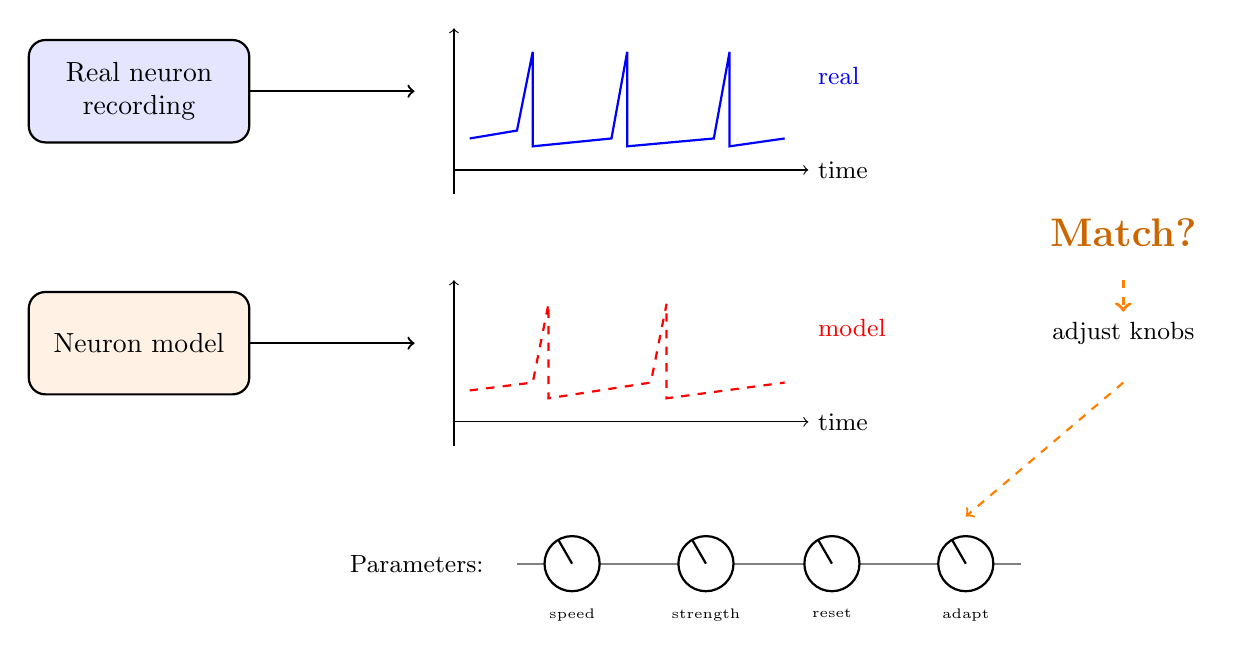
\begin{tikzpicture}[
    box/.style={draw, rounded corners=6pt, minimum width=2.8cm, minimum height=1.3cm,
                align=center, font=\normalsize, thick}
]
    
    \begin{scope}[xshift=-4cm, yshift=1cm]
        % Real neuron recording
        \node[box, fill=blue!10] (real) at (0,2.2) {Real neuron\\recording};

        % Model with knobs
        \node[box, fill=orange!10] (model) at (0,-1) {Neuron model};
    \end{scope}

    \begin{scope}[xshift=4cm, yshift=0cm]
    % Parameter knobs
    \draw[thick, gray] (-3.2,-2.8) -- (3.2,-2.8);
    \foreach \x/\lab in {-2.5/speed, -0.8/strength, 0.8/reset, 2.5/adapt} {
        \draw[thick, fill=white] (\x,-2.8) circle (0.35);
        \draw[thick, rotate around={30:(\x,-2.8)}] (\x,-2.8) -- ++(0,0.35);
        \node[font=\tiny, below] at (\x,-3.25) {\lab};
    }
    \node[font=\small, left] at (-3.5,-2.8) {Parameters:};
    \end{scope}

    % Output traces
    \begin{scope}[xshift=0cm, yshift=2.2cm]
        \draw[->] (0,0) -- (4.5,0) node[right, font=\small] {time};
        \draw[->] (0,-0.3) -- (0,1.8);
        \draw[blue, thick] (0.2,0.4) -- (0.8,0.5) -- (1,1.5) -- (1,0.3) -- (2,0.4) -- (2.2,1.5) -- (2.2,0.3) -- (3.3,0.4) -- (3.5,1.5) -- (3.5,0.3) -- (4.2,0.4);
        \node[blue, font=\small, right] at (4.5,1.2) {real};
    \end{scope}

    \begin{scope}[xshift=0cm, yshift=-1cm]
        \draw[->] (0,0) -- (4.5,0) node[right, font=\small] {time};
        \draw[->] (0,-0.3) -- (0,1.8);
        \draw[red, thick, dashed] (0.2,0.4) -- (1.0,0.5) -- (1.2,1.5) -- (1.2,0.3) -- (2.5,0.5) -- (2.7,1.5) -- (2.7,0.3) -- (4.2,0.5);
        \node[red, font=\small, right] at (4.5,1.2) {model};
    \end{scope}

    % Arrows
    \draw[->, thick] (real) -- ++(3.5,0);
    \draw[->, thick] (model) -- ++(3.5,0);

    % Question
    \node[font=\Large, orange!80!black] at (8.5,1.4) {\textbf{Match?}};

    % Goal arrow
    \draw[->, very thick, orange, dashed] (8.5,0.8) -- (8.5, 0.4) node[below, font=\small, text=black] {adjust knobs};
    \draw[->, thick, orange, dashed] (8.5, -0.5) -- (6.5,-2.2);
\end{tikzpicture}
\end{center}

\vspace{0.2cm}
\centering
\large \textbf{Goal:} Automatically find the right parameter settings
\end{frame}

%% ============================================================
%% SLIDE 3: The Cliff — Why this is hard
%% ============================================================
\begin{frame}{The Obstacle: Spikes Break the Math}
\begin{columns}[c]
\begin{column}{0.52\textwidth}
\begin{center}
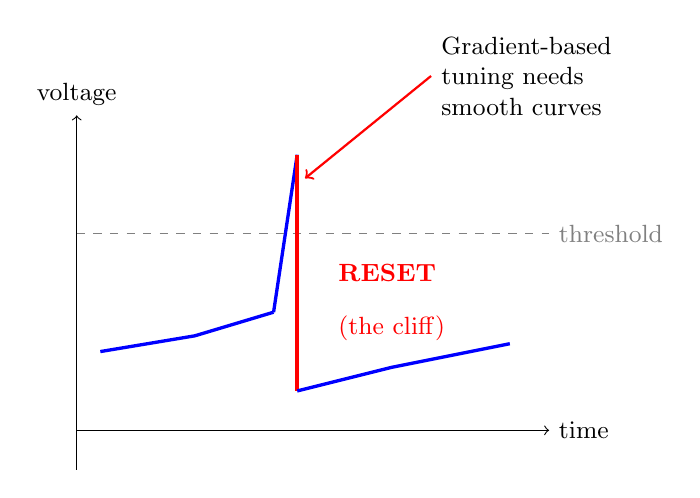
\begin{tikzpicture}[scale=1.0]
    % Voltage trace with spike
    \draw[->] (0,0) -- (6,0) node[right, font=\small] {time};
    \draw[->] (0,-0.5) -- (0,4) node[above, font=\small] {voltage};

    % Subthreshold
    \draw[blue, very thick] (0.3,1) -- (1.5,1.2) -- (2.5,1.5);

    % Spike up
    \draw[blue, very thick] (2.5,1.5) -- (2.8,3.5);

    % Threshold line
    \draw[dashed, gray] (0,2.5) -- (6,2.5);
    \node[gray, font=\small, right] at (6,2.5) {threshold};

    % Reset — the cliff!
    \draw[red, ultra thick] (2.8,3.5) -- (2.8,0.5);
    \node[red, font=\small, right] at (3.2,2.0) {\textbf{RESET}};
    \node[red, font=\small, right] at (3.2,1.3) {(the cliff)};

    % Continue
    \draw[blue, very thick] (2.8,0.5) -- (4,0.8) -- (5.5,1.1);

    % Annotation
    \draw[<-, thick, red] (2.9,3.2) -- (4.5,4.5) node[right, font=\small, text=black, align=left] {Gradient-based\\tuning needs\\smooth curves};
\end{tikzpicture}
\end{center}
\end{column}
\begin{column}{0.45\textwidth}
\begin{center}
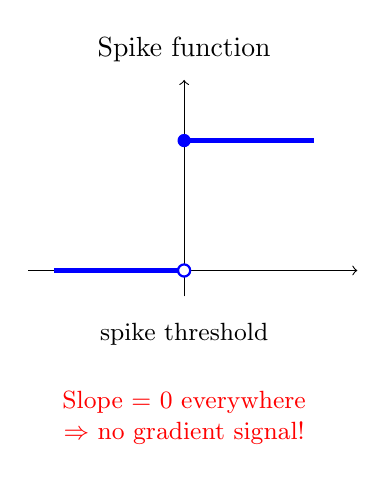
\begin{tikzpicture}[scale=1.1]
    % Heaviside
    \draw[->] (-1.8,0) -- (2,0);
    \draw[->] (0,-0.3) -- (0,2.2);

    \draw[blue, ultra thick] (-1.5,0) -- (0,0);
    \draw[blue, ultra thick] (0,1.5) -- (1.5,1.5);
    \draw[blue, fill=white, thick] (0,0) circle (0.07);
    \draw[blue, fill=blue] (0,1.5) circle (0.07);

    \node[font=\small, below] at (0,-0.5) {spike threshold};
    \node[font=\normalsize, above, align=center] at (0,2.3) {Spike function};

    % Gradient = 0 annotation
    \node[red, font=\small, align=center] at (0,-1.7) {Slope = 0 everywhere\\$\Rightarrow$ no gradient signal!};
\end{tikzpicture}
\end{center}
\end{column}
\end{columns}

\vspace{0.4cm}
\centering
\large Gradient-based tuning is fast --- but needs smooth functions.\\
Spikes create a \alert{cliff} that blocks the gradient.
\end{frame}

%% ============================================================
%% SLIDE 4: The Fix — Surrogate Gradients
%% ============================================================
\begin{frame}{The Trick: Surrogate Gradients}
\begin{columns}[c]
\begin{column}{0.45\textwidth}
\begin{center}
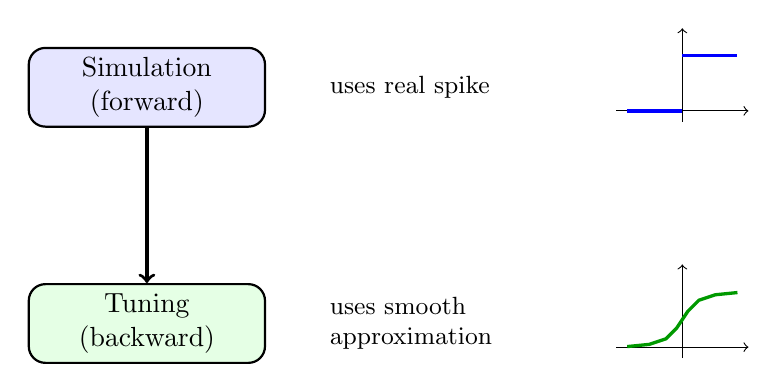
\begin{tikzpicture}[
    box/.style={draw, rounded corners=6pt, minimum width=3cm, minimum height=1cm,
                align=center, font=\normalsize, thick}
]
    \node[box, fill=blue!10] (fwd) at (0,2) {Simulation\\(forward)};
    \node[box, fill=green!10] (bwd) at (0,-1) {Tuning\\(backward)};

    \node[font=\small, right, align=left] at (2.2,2) {uses real spike};
    \node[font=\small, right, align=left] at (2.2,-1) {uses smooth\\ approximation};

    % Mini step function
    \begin{scope}[xshift=6.8cm, yshift=1.7cm, scale=0.7]
        \draw[->] (-1.2,0) -- (1.2,0);
        \draw[->] (0,-0.2) -- (0,1.5);
        \draw[blue, very thick] (-1,0) -- (0,0);
        \draw[blue, very thick] (0,1) -- (1,1);
    \end{scope}

    % Mini smooth function — piecewise linear approximation of sigmoid
    \begin{scope}[xshift=6.8cm, yshift=-1.3cm, scale=0.7]
        \draw[->] (-1.2,0) -- (1.2,0);
        \draw[->] (0,-0.2) -- (0,1.5);
        \draw[green!60!black, very thick]
            (-1,0.01) -- (-0.6,0.05) -- (-0.3,0.15) -- (-0.1,0.35) -- (0,0.5)
            -- (0.1,0.65) -- (0.3,0.85) -- (0.6,0.95) -- (1,0.99);
    \end{scope}

    \draw[->, very thick] (fwd) -- (bwd);
\end{tikzpicture}
\end{center}
\end{column}
\begin{column}{0.50\textwidth}
\begin{center}

\includegraphics[width=\textwidth]{figures/surrogate_gradients_comparison.pdf}
\end{center}
\end{column}
\end{columns}

\vspace{0.5cm}
\centering
\large \textbf{Key idea:} Keep the real spike for simulation,\\
use a smooth stand-in for tuning.
\end{frame}

%% ============================================================
%% SLIDE 5: The Real Challenge — Loss Functions (compass)
%% ============================================================
\begin{frame}{The Real Challenge: Measuring ``How Wrong''}
\begin{columns}[c]
\begin{column}{0.50\textwidth}
\begin{center}
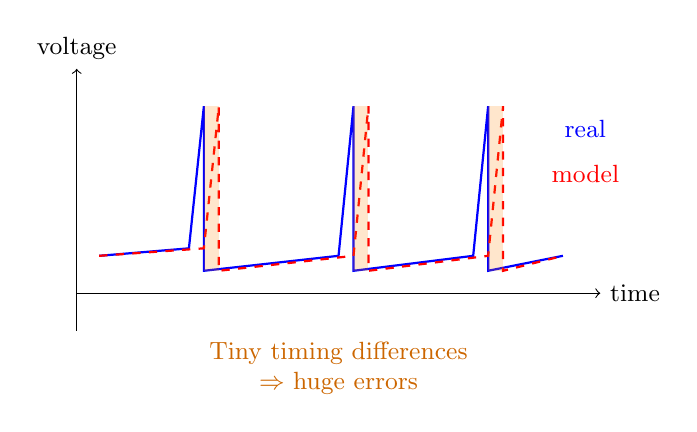
\begin{tikzpicture}[scale=0.95]
    % Two traces
    \draw[->] (0,0) -- (7,0) node[right, font=\small] {time};
    \draw[->] (0,-0.5) -- (0,3) node[above, font=\small] {voltage};

    % Real trace
    \draw[blue, thick] (0.3,0.5) -- (1.5,0.6) -- (1.7,2.5) -- (1.7,0.3) -- (3.5,0.5) -- (3.7,2.5) -- (3.7,0.3) -- (5.3,0.5) -- (5.5,2.5) -- (5.5,0.3) -- (6.5,0.5);

    % Model trace (slightly offset)
    \draw[red, thick, dashed] (0.3,0.5) -- (1.7,0.6) -- (1.9,2.5) -- (1.9,0.3) -- (3.7,0.5) -- (3.9,2.5) -- (3.9,0.3) -- (5.5,0.5) -- (5.7,2.5) -- (5.7,0.3) -- (6.5,0.5);

    \node[blue, font=\small] at (6.8,2.2) {real};
    \node[red, font=\small] at (6.8,1.6) {model};

    % Error highlight
    \fill[orange, opacity=0.2] (1.7,0.3) rectangle (1.9,2.5);
    \fill[orange, opacity=0.2] (3.7,0.3) rectangle (3.9,2.5);
    \fill[orange, opacity=0.2] (5.5,0.3) rectangle (5.7,2.5);

    % Annotation
    \node[orange!80!black, font=\small, align=center] at (3.5,-1) {Tiny timing differences\\$\Rightarrow$ huge errors};
\end{tikzpicture}
\end{center}
\end{column}
\begin{column}{0.45\textwidth}
\vspace{-0.3cm}
\begin{center}
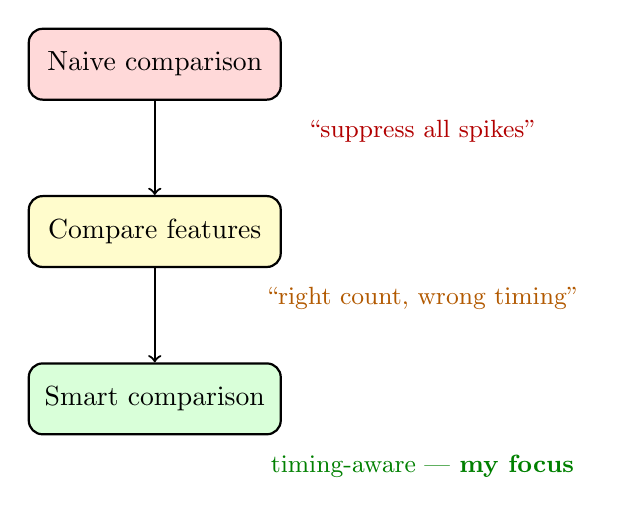
\begin{tikzpicture}[
    scale=0.85,
    box/.style={draw, rounded corners=5pt, minimum width=3.2cm, minimum height=0.9cm,
                align=center, font=\normalsize, thick}
]
    \node[box, fill=red!15] (naive) at (0,2.5) {Naive comparison};
    \node[font=\small, red!70!black] at (4,1.5) {``suppress all spikes''};

    \node[box, fill=yellow!20] (feat) at (0,0) {Compare features};
    \node[font=\small, orange!70!black] at (4,-1) {``right count, wrong timing''};

    \node[box, fill=green!15] (smart) at (0,-2.5) {Smart comparison};
    \node[font=\small, green!50!black] at (4,-3.5) {timing-aware --- \textbf{my focus}};

    \draw[->, thick] (naive) -- (feat);
    \draw[->, thick] (feat) -- (smart);
\end{tikzpicture}
\end{center}
\end{column}
\end{columns}

\vspace{0.3cm}
\centering
\large Gradients tell you \emph{how} to adjust --- the loss function tells you \emph{where} to go.\\
A bad compass leads you astray, no matter how fast you walk.
\end{frame}

%% ============================================================
%% SLIDE 6: Why It Matters
%% ============================================================
\begin{frame}{Why It Matters}
\begin{center}
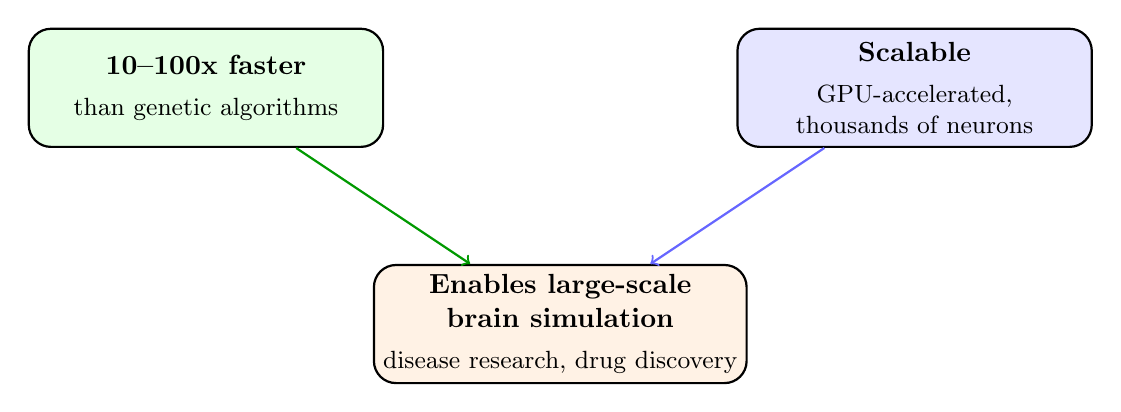
\begin{tikzpicture}[
    box/.style={draw, rounded corners=8pt, minimum width=4.5cm, minimum height=1.5cm,
                align=center, font=\normalsize, thick}
]
    \node[box, fill=green!10] (fast) at (-4.5,1.5) {
        \textbf{10--100x faster}\\[3pt]
        \small than genetic algorithms
    };

    \node[box, fill=blue!10] (scale) at (4.5,1.5) {
        \textbf{Scalable}\\[3pt]
        \small GPU-accelerated,\\[-1pt]
        \small thousands of neurons
    };

    \node[box, fill=orange!10] (brain) at (0,-1.5) {
        \textbf{Enables large-scale}\\
        \textbf{brain simulation}\\[3pt]
        \small disease research, drug discovery
    };

    \draw[->, thick, green!60!black] (fast) -- (brain);
    \draw[->, thick, blue!60] (scale) -- (brain);
\end{tikzpicture}
\end{center}

\vspace{0.8cm}
\centering
\Large If we can make gradient-based tuning work for simplified models,\\
we unlock \textbf{faster and larger} brain simulations.
\end{frame}

\end{document}
